\section{Ensemble Methods}
\begin{highlight}{Bagging vs. Boosting}
\begin{tabular}{ p{0.45\columnwidth} | p{0.45\columnwidth} }
		\textbf{Bagging} & \textbf{Boosting}\\\hline
		 trains learners in parallel and combines them using deterministic averaging. & trains learners sequentially in an adaptive way and combines them using a deterministic strategy. \\\hline
  		 less variance than the components & less biased than the components 
\end{tabular}



\end{highlight}
Combination of multiple weak learners to get a stronger learner. (Wisdom of crowds)
\subsection{Bagging}
\begin{enumerate}
	\item Bootstrap sets: Draw $M$ bootstrap sets
	\item Train $M$ base models $b^{(1)}, ... , b^{(M)}$
	\item Aggregate 
	$$	\bbar =
		\begin{cases}
			\frac{1}{M}\sum_{t\leq M} b^{(t)}(x) &\text{regression}\\
			\textit{majority}\left(b^{(t)}(x)\right)_{t\leq M}&\text{classification}
		\end{cases}
	$$
\end{enumerate}
\begin{center}
	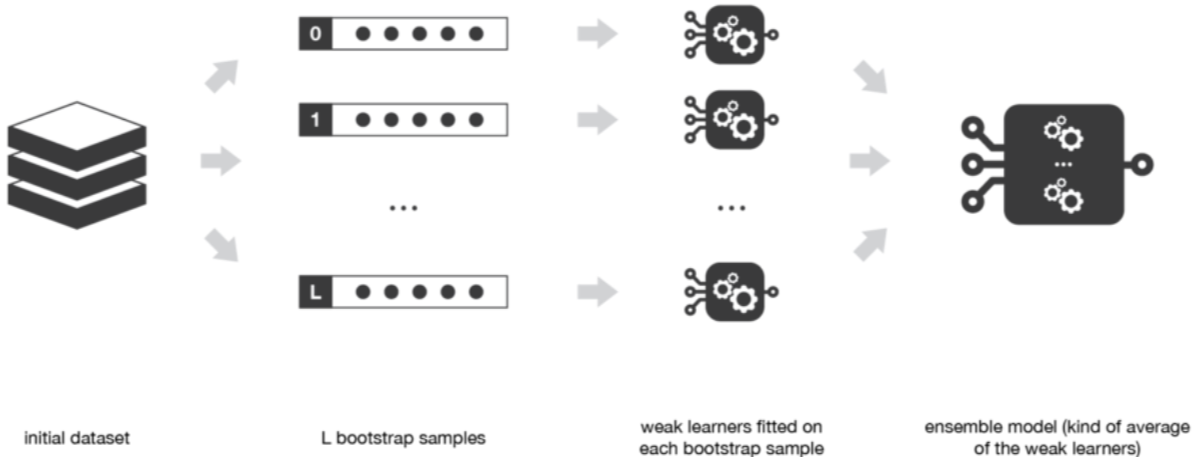
\includegraphics[width=\columnwidth]{images/9-bagging}
\end{center}

\textbf{Theorem}: For $x\in \mathcal X$ if $range(y) < \infty$, then there is a sufficiently large $M$ s.t. $\E[(y - \bar{b}^{(M)}(x))^2] \leq \E[(y - b(x))^2]$ for some base model $b$.

\textit{Proof in Slides, p.20-21}


\textbf{Properties of the base models}
\begin{itemize}
	\item Diversity
	\item Independence: Bootstrap sets should be independent, but \textbf{they are not} (but correlation is small).
\end{itemize}



\subsubsection{Random forests}
\textit{The \href{https://towardsdatascience.com/ensemble-methods-bagging-boosting-and-stacking-c9214a10a205}{Random forest} method is a bagging method with trees as weak learners. Each tree is fitted on a bootstrap sample considering only a \textbf{subset of variables} randomly chosen. This helps \textbf{reduce the correlation} between trained base trees in the ensemble.
}
\begin{center}
	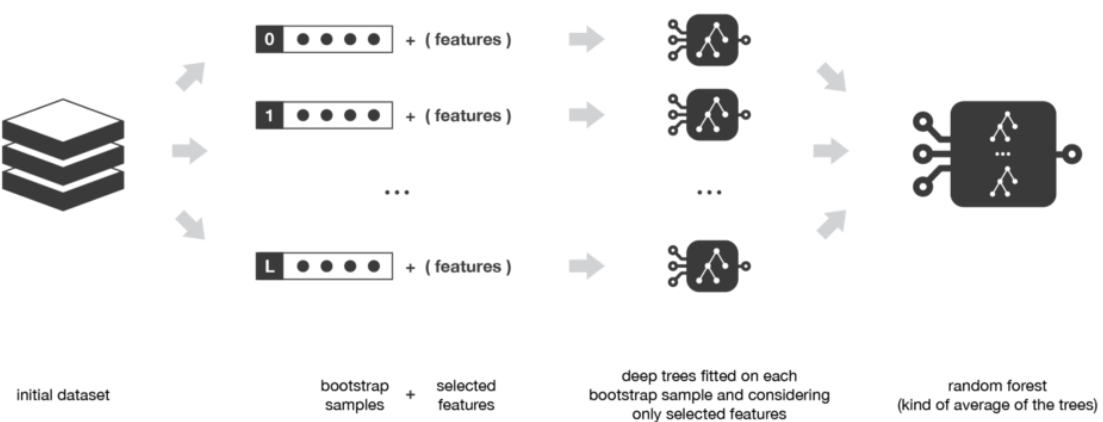
\includegraphics[width=\columnwidth]{images/9-random-forests}
\end{center}





\subsection{Boosting }
\textit{Key: Learning from previous mistakes.}

Fit models iteratively, such that the training of the model at a given step depends on the models fitted in previous steps. Each model gives higher weight to the observations that were handled badly in the previous steps.


\begin{center}
	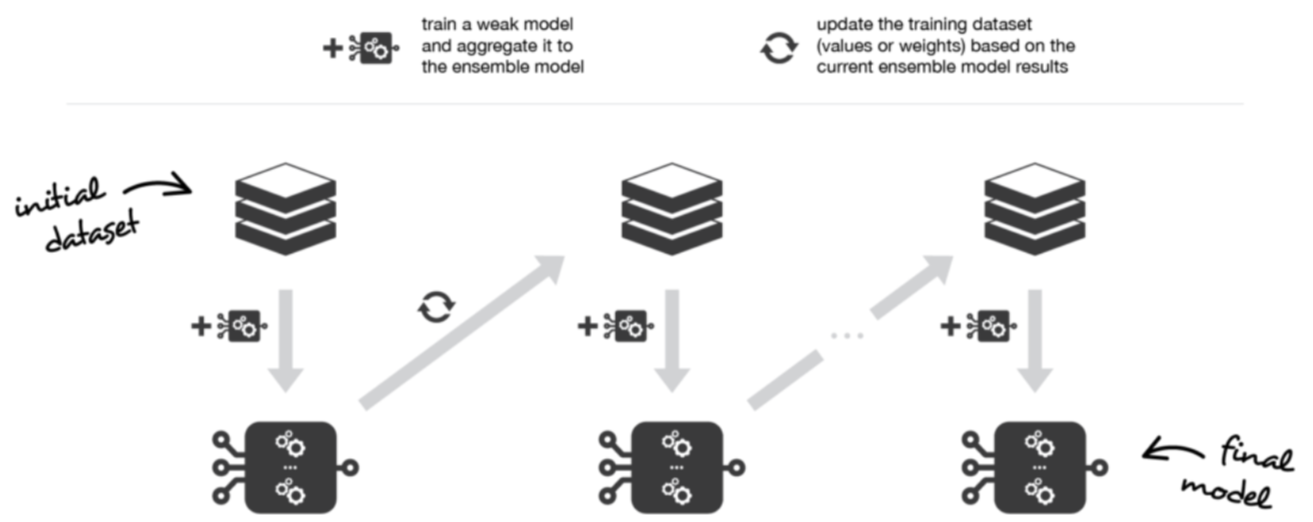
\includegraphics[width=0\columnwidth]{images/9-boosting}
\end{center}


\subsubsection{Ada Boost (Adaptive Boosting)}
\textit{Learn from previous mistakes by increasing the weight of misclassified datapoints. \textbf{Outliers} will get very high weights and can be detected by that.
}\begin{itemize}
	\item Loss function: $0$-$1$ Loss
	\item Base models (stumps)
	\item place high weights on samples that are very hard to classify
\end{itemize}



Let $\mathcal L^{(w)} = \sumin w_i * \mathds{1} \{b(x_i)\neq y_i\}$ (the 0-1 loss)

\begin{algorithm}[H]  
	\tcp{Initialize}
	$\bbar^{(0)} \gets 0$ \\ 
	$w_i \gets 1/n$ for $i\leq n$ \\
	\For{t=1..M}{
		\tcp{Train}
		$b^{(t)} \gets \arg\min_b \L^{(w)}(b)$\\ 
		\vspace{1em}
		\tcp{Evaluate}
		$err_t \gets \mathcal L^{(w)}(b^{(t)})$\\
		\vspace{1em}
		\tcp{Reweigh}
		$w_i \gets
			\begin{cases}
				\tilde\alpha_tw_i &\textit{if }b^{(t)}(x_i)\neq y_i \textit{ for } i\leq n, \tilde\alpha_t = \frac{1}{err_t}-1 \\
				w_i &\textit{otherwise }
			\end{cases}$ \\
		\vspace{1em}
		\tcp{Add to set}
		$\bbar \gets \bbar^{(t-1)} + \tilde \alpha_t b^{(t)}$\\
		\vspace{1em}

		\textit{normalize}($ w_1, ... ,w_n$)\\
	}
	\caption{AdaBoost Algorithm}
\end{algorithm}


\textbf{AdaBoost for Classification: } 
\begin{enumerate}
	\item Train $\alpha_1, b^{(1)}, ..., \alpha_M, b^{(M)}$
	\begin{equation*}
		\begin{gathered}
					\alpha_1, b^{(1)}, ..., \alpha_M, b^{(M)} \\
			\alpha_t \in [0, \infty) \\
			b^{(t)}: \mathcal X \to \{-1, +1\}
		\end{gathered}
	\end{equation*} 
	\item predict $\bbar^{(M)} = sgn(\sum_{t\leq M}\alpha_tb^{(t)}(x))$
\end{enumerate}

\textbf{Why is AdaBoost so successful?}
\textit{Theoretical results: Slides p. 57-}
\begin{itemize}
	\item Friedmann: AdaBoost is equal to forward additive stepwise modeling (FSAM) with exponential loss
		\item Boosting trains max-margin classifiers
	\item Wyner et al: AdaBoost and random forest train spiky, interpolating and self-averaging models.
	
	\begin{minipage}{0.35\columnwidth}
	\textbf{Spiky: }
	\begin{center}
		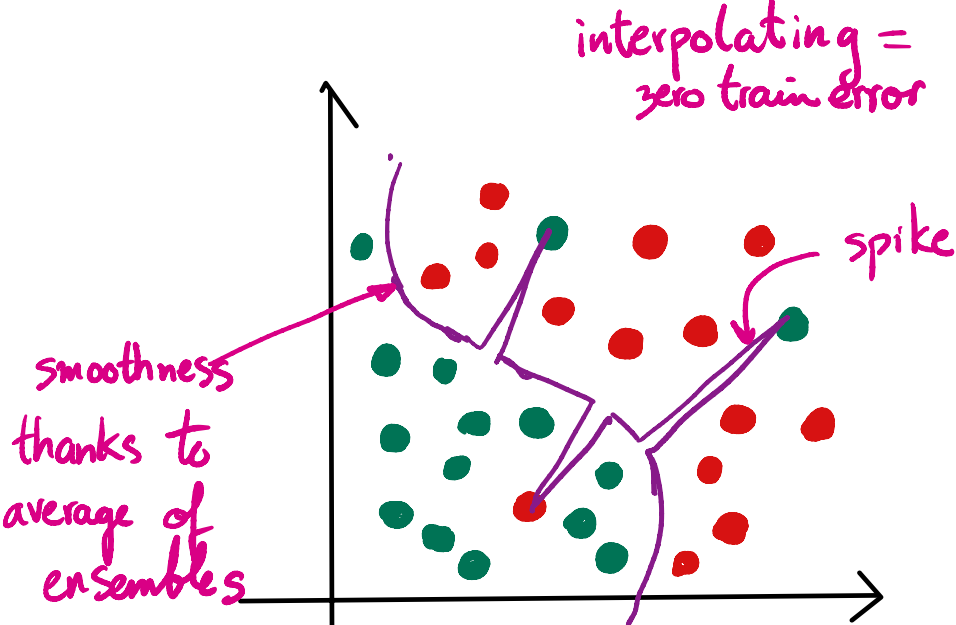
\includegraphics[width=\columnwidth]{images/9-adaboost-spiky}
	\end{center}
	\end{minipage}
	\begin{minipage}{0.55\columnwidth}
		\begin{itemize}
			\item Mostly smooth with Sharp localized changes to interpolate noisy examples
			\item This prevents influence from noise and allows fitting of complex signals.
		\end{itemize}
	\end{minipage}
	
	\begin{minipage}{0.35\columnwidth}
	\textbf{Self-Averaging: }
	\begin{center}
		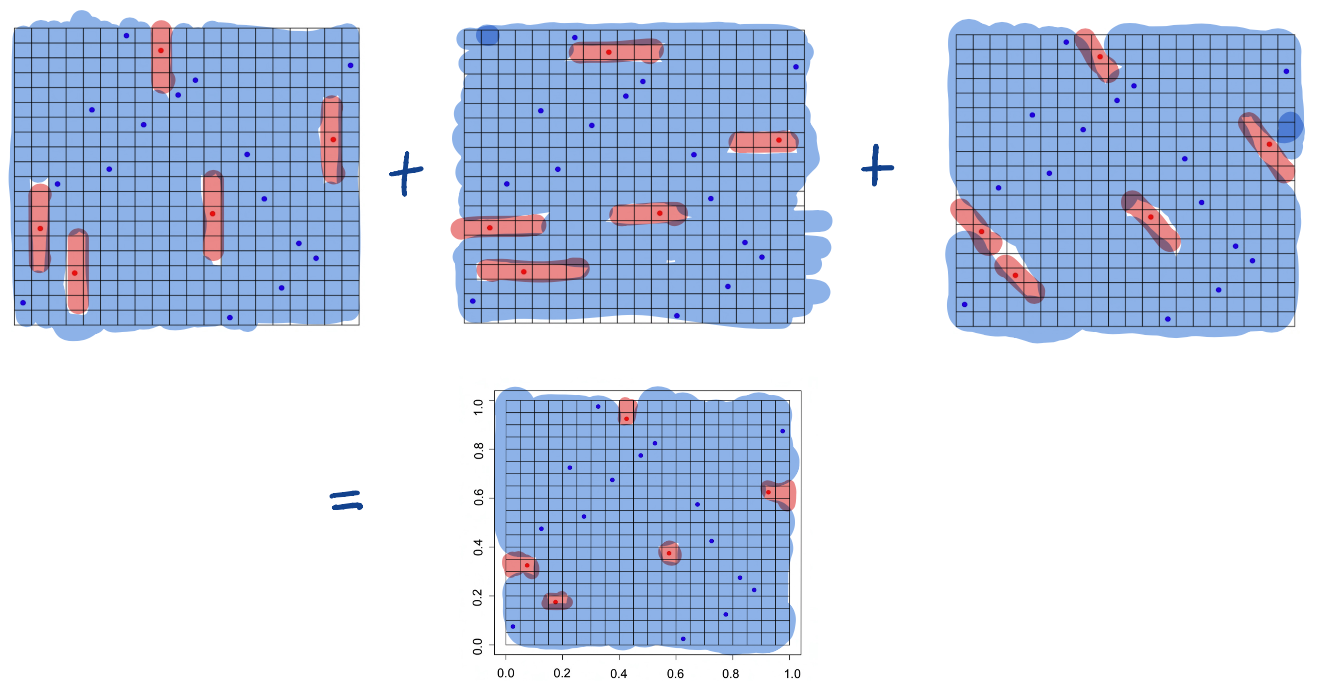
\includegraphics[width=\columnwidth]{images/9-adaboost-selfavg}
	\end{center}
	\end{minipage}
	\begin{minipage}{0.55\columnwidth}
		\begin{itemize}
			\item Trained model is an average of diverse models
			\item Averaging spiky interpolation helps localise noisy effects
		\end{itemize}
	\end{minipage}	
\end{itemize}

\begin{minipage}{\columnwidth}
	\textbf{AdaBoost with complex base classifiers trains spiky interpolation classifiers.}



\begin{tabular}{p{0.2\columnwidth} | p{0.2\columnwidth} | p{0.2\columnwidth} | p{0.2\columnwidth}}
		\textbf{base classif.} & \textbf{Vertical Stumps} & \textbf{Stumps} & \textbf{Full Trees}\\\hline
		\textbf{Trained Ensemble}
		&
  		\begin{center}
  		\vspace{-1em}
			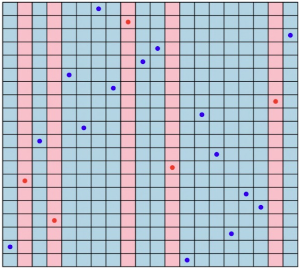
\includegraphics[width=0.2\columnwidth]{images/9-adaboost-baseclassif-1}
		\end{center} &  
		\begin{center}
  		\vspace{-1em}
			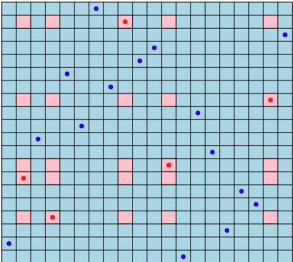
\includegraphics[width=0.2\columnwidth]{images/9-adaboost-baseclassif-2}
		\end{center}
  		& 
  		\begin{center}
  		\vspace{-1em}
			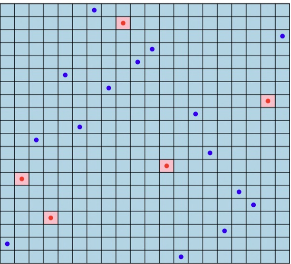
\includegraphics[width=0.2\columnwidth]{images/9-adaboost-baseclassif-3}
		\end{center} \\\hline
		\textbf{gen. error} & high & medium & low \\\hline
		\textbf{Interp.} & $\checkmark$ & $\checkmark$ & $\checkmark$ \\\hline
		\textbf{spiky} & $\times$ & $\sim$ & $\checkmark$ \\\hline
\end{tabular}
\end{minipage}

\subsubsection{Gradient Boosting}
\textit{Similarly to AdaBoost, gradient Boosting is a\textbf{ method to greedily approximate $f$} using gradient descent based on the additive form. Gradient Boosting learns directly from the residual error instead of updating the weights. }
\begin{equation*}
	f_M(x) = \sumi M \beta_i h_i(x), \textit{where $h_i$ are the weak learners.}
\end{equation*}

\begin{algorithm}[H]  
	$\hat f_0(\x) = \argmin_h \sumi n L(y_i, h(\x_i)$\tcp*[r]{Init}
	\For{t=1..M}{
	\tcp{Compute the negative gradient :} 
		$-g_m(\x_i) = \left[\frac{\partial L(y_i, f(\x_i))}{\partial f(\x_i)} \right]_{f = \hat f_{m-1}(\x_i)}, i= 1... n$ \\\vspace{1em}

		\tcp{Fit function $h_m$ to negative gradient by least squares: } 
		$h_m = \argmin_h\sumi n(-g_m(\x_i - h(\x_i))^2$ \\\vspace{1em}

		\tcp{Find $\beta_m$ to minimize the loss } 
		$\beta_m = \argmin_\beta\sumi n L(y_i, \hat f_{m-1}(\x_i) - h(\x_i))^2$\\\vspace{1em}
		
		\tcp{Update $\hat f$} 
		$\hat f_m(\x) = \hat f_{m-1} + \beta_mh_m(\x)$
	}
	\caption{Gradient Boosting algorithm}
\end{algorithm}

\textbf{Differences AdaBoost / Gradient Boosting: }
\begin{itemize}
	\item AdaBoost learns from mistake by increasing the weight of misclassified data-points.
	\item Gradient Boosting learns from the residual error (mistake) directly instead of updating weights.
\end{itemize}


\subsubsection{Forward Stagewise Additive Modeling (Exercise 6)}
Method to approximately compute a classifier of the form $c(x) = \mathit{sgn}(\sum_t\alpha_t b^{(t)}$ that approximately minimizes the empirical loss $\sumin L(y_i, c(x_i))$.

\begin{algorithm}[H]  
	\SetKwInOut{Input}{input}
	\SetKwInOut{Output}{output}
	
	\Input{
		\begin{itemize}
			\item $\{(x_1, y_1), ..., (x_n, y_n)\}\subseteq\R^D\times \{-1, 1\}$
			\item $L:\{1, -1\}\times \{1, -1\}\to \R$
			\item $M\in \N$
		\end{itemize}
	}
	\Output{$\hat c \approx \argmin_c \sumi n L(y_i, c(x_i))$} 
	\vspace{1em}
	
	$f_0(x) \gets 0 \forall x\in\R^D$ \\
	\For{$t=1$ to $M$}{
		$(\alpha_t, b^{(t)}) \gets \argmin_{\substack{\alpha > 0 \\ b\in\mathcal H}} \sumi n L(y_i, \alpha b(x_i) + f_{t-1}(x_i))$ \\
		$f_t(x) \gets \alpha_tb^{(t)}(x) + f_{t-1}(x) \forall x\in\R^D$ \\
	}
	\Return{$\hat c \gets \mathit{sgn}(f_M(x)) \forall x\in\R^D$}
	\caption{Forward stagewise additive modeling}
\end{algorithm}

$\Rightarrow$ \textbf{Exercise 1: AdaBoost is equivalent to forward stagewise additive modeling}
